% Options for packages loaded elsewhere
\PassOptionsToPackage{unicode}{hyperref}
\PassOptionsToPackage{hyphens}{url}
%
\documentclass[
]{article}
\usepackage{lmodern}
\usepackage{amssymb,amsmath}
\usepackage{ifxetex,ifluatex}
\ifnum 0\ifxetex 1\fi\ifluatex 1\fi=0 % if pdftex
  \usepackage[T1]{fontenc}
  \usepackage[utf8]{inputenc}
  \usepackage{textcomp} % provide euro and other symbols
\else % if luatex or xetex
  \usepackage{unicode-math}
  \defaultfontfeatures{Scale=MatchLowercase}
  \defaultfontfeatures[\rmfamily]{Ligatures=TeX,Scale=1}
\fi
% Use upquote if available, for straight quotes in verbatim environments
\IfFileExists{upquote.sty}{\usepackage{upquote}}{}
\IfFileExists{microtype.sty}{% use microtype if available
  \usepackage[]{microtype}
  \UseMicrotypeSet[protrusion]{basicmath} % disable protrusion for tt fonts
}{}
\makeatletter
\@ifundefined{KOMAClassName}{% if non-KOMA class
  \IfFileExists{parskip.sty}{%
    \usepackage{parskip}
  }{% else
    \setlength{\parindent}{0pt}
    \setlength{\parskip}{6pt plus 2pt minus 1pt}}
}{% if KOMA class
  \KOMAoptions{parskip=half}}
\makeatother
\usepackage{xcolor}
\IfFileExists{xurl.sty}{\usepackage{xurl}}{} % add URL line breaks if available
\IfFileExists{bookmark.sty}{\usepackage{bookmark}}{\usepackage{hyperref}}
\hypersetup{
  hidelinks,
  pdfcreator={LaTeX via pandoc}}
\urlstyle{same} % disable monospaced font for URLs
\usepackage{graphicx}
\makeatletter
\def\maxwidth{\ifdim\Gin@nat@width>\linewidth\linewidth\else\Gin@nat@width\fi}
\def\maxheight{\ifdim\Gin@nat@height>\textheight\textheight\else\Gin@nat@height\fi}
\makeatother
% Scale images if necessary, so that they will not overflow the page
% margins by default, and it is still possible to overwrite the defaults
% using explicit options in \includegraphics[width, height, ...]{}
\setkeys{Gin}{width=\maxwidth,height=\maxheight,keepaspectratio}
% Set default figure placement to htbp
\makeatletter
\def\fps@figure{htbp}
\makeatother
\setlength{\emergencystretch}{3em} % prevent overfull lines
\providecommand{\tightlist}{%
  \setlength{\itemsep}{0pt}\setlength{\parskip}{0pt}}
\setcounter{secnumdepth}{-\maxdimen} % remove section numbering
\usepackage{fancyvrb,newverbs,xcolor} % for code highlighting
\usepackage[top=2cm, bottom=1.5cm, left=2cm, right=2cm]{geometry} % for page margins

\usepackage[english]{babel}
% Ana: adding graphics package for images
\usepackage{graphics}
\usepackage{graphicx}

% change background color for inline code in
% markdown files. The following code does not work well for
% long text as the text will exceed the page boundary
%\definecolor{bgcolor}{HTML}{E0E0E0}
%\let\oldtexttt\texttt

% \renewcommand{\texttt}[1]{
% \colorbox{bgcolor}{\oldtexttt{#1}}
% }


%% Setting pythong ??? -----------------------------------------------------
%default_block_language: "lexer"
%default_inline_language: "lexer"


%% color and other settings for hyperref package -----------------------------
\hypersetup{
    bookmarksopen=true,
    linkcolor=blue,
    filecolor=magenta,
    urlcolor=RoyalBlue,
}

% Font Setup  ---------------------------------------------------------
\usepackage{unicode-math} % load 'fontspec' automatically
\setmainfont{Crimson}
%\setmainfont{Libertinus Sans} 
%\setmainfont{Alegreya}
\setmathfont{TeX Gyre Schola Math}


% Code syntax highlighting ---------------------------------------------------

% OLD PART -----------------
%\usepackage{minted}
%\usemintedstyle{manni}
%\setmonofont{Inconsolata}
% ---------------------------


% Preliminary macro things for code (snatched from macros in REPORT):  ------
\newcommand\CodeFontSizeSmall{\fontsize{9pt}{9pt}\selectfont}

\definecolor{originalmannibg}{HTML}{f2f2ff}
\colorlet{BasePurple}{originalmannibg!90}
\newcommand{\lighten}[3]{% Reference Color, Percentage, New Color Name
    \colorlet{#3}{#1!#2!white}
}
\lighten{BasePurple}{50}{mannibg}

% Code things --------------------
\usepackage{minted}
\usepackage{verbatim}  % has commenting



\usemintedstyle{manni}

%\setmonofont{Inconsolata} % setting code font
\setmonofont{Fira Mono}

% General code environment, used like: \begin{code}{python} .... \end{code}
% NOTE: this is how to nest two environments together: 
\newenvironment{code}[2][]
 {\vspace{-3pt}%
 \VerbatimEnvironment
  \begin{adjustwidth}{30pt}{30pt}
  \begin{minted}[
    fontsize=\CodeFontSizeSmall,
    breaklines, mathescape,
    style=manni, bgcolor=mannibg,  #1]{#2}}
 {\end{minted}\end{adjustwidth} 
     \vspace{-10pt}
 }
 
% TODO: test if possible to do \renewenvironment to renew the minted environment and just include this logic below whenever calling \begin{minted}[]{python} ... 
 
% Python code environment, used like \begin{pythonCode} ... \end{pythonCode}
\newenvironment{pythonCode}
 {\vspace{-3pt}%
 \VerbatimEnvironment
  \begin{adjustwidth}{30pt}{30pt}
  \begin{minted}[
    fontsize=\CodeFontSizeSmall,
    breaklines, mathescape,
    style=manni, bgcolor=mannibg]{python}}
 {\end{minted}\end{adjustwidth} 
     \vspace{-10pt}
 }



% General code output environment
\newenvironment{outputCode}
 {\VerbatimEnvironment
  \begin{adjustwidth}{30pt}{30pt}
  \begin{minted}[
    fontsize=\CodeFontSizeSmall,
    breaklines]{text}}
 {\end{minted}\end{adjustwidth}}


% Creating inline code font (equivalent to backticks in jupyter notebooks)
% Must use like: \pythoninline{...text here ... }
\newmintinline{python}{python3, fontsize=\CodeFontSizeSmall, bgcolor=mannibg}

%\newenvironment{mintInline}[1][]{\mintinline{latex}{#1}}{}
%\DeclareTextFontCommand{\mint}{\mintInline}



\author{}
\date{}

\begin{document}

Source:
https://github.com/explosion/thinc/blob/master/examples/05\_visualizing\_models.ipynb

\hypertarget{visualizing-thinc-models-with-shape-inference}{%
\section{Visualizing Thinc Models (with shape
inference)}\label{visualizing-thinc-models-with-shape-inference}}

\textbf{Goal}: to visualize Thinc models and their inputs and outputs.

\hypertarget{define-the-model}{%
\subsection{1. Define the Model}\label{define-the-model}}

Start by defining the model with a number of layers chained together
using the \mintinline[]{python}{chain} combinator.

\begin{minted}[]{python}
from typing import Dict, Any

from pydot import Dot, Node
from thinc.api import chain, expand_window, Relu, Maxout, Linear, Softmax, Model

numHidden: int = 32
dropout: float = 0.2

model: Model = chain(
    expand_window(window_size = 3),
    Relu(nO = numHidden, dropout = dropout, normalize = True),
    Maxout(nO = numHidden * 4),
    Linear(nO = numHidden * 2),
    Relu(nO = numHidden, dropout = dropout, normalize = True),
    Linear(nO = numHidden),
    Relu(nO = numHidden, dropout = dropout),
    Softmax(),
)
\end{minted}

\begin{minted}[]{python}
model
\end{minted}

\begin{minted}[]{python}
<thinc.model.Model at 0x7f978417da60>
\end{minted}

\hypertarget{visualizing-the-model}{%
\subsection{2. Visualizing the model}\label{visualizing-the-model}}

Must add a node for each layer, edges connecting the nodes to the
previous enode (except for first/last), and labels like
``\mintinline[]{python}{name | (nO, nI)}'', for instance
``\mintinline[]{python}{maxout | (128, 32)}''.

Function below takes a Thinc layer (such as a
\mintinline[]{python}{Model} instance) and returns a label with the
layer name and its dimensions, if available:

\begin{minted}[]{python}
import thinc

# todo: type?
def getLabel(layer) -> str:
    # todo type
    layerName = layer.name
    nO: int = layer.get_dim("nO") if layer.has_dim("nO") else "?"
    nI: int = layer.get_dim("nI") if layer.has_dim("nI") else "?"

    return f"{layer.name}|({nO}, {nI})".replace(">", "&gt;")
\end{minted}

Can now use \mintinline[]{python}{pydot} to create a visualization for a
given model. Can customize the direction of the notes by setting
``\mintinline[]{python}{rankdir}'' (e.g.~specifying
``\mintinline[]{python}{TB}'' for ``top to bottom'') and adjust the font
and arrow styling. Call IPython's utilities so visualization renders
nicely in the notebook.

\begin{minted}[]{python}
import pydot

#from pydot import Dot
from IPython.display import SVG, display


def visualizeModel(model: Model):

    dot: Dot = pydot.Dot()

    # Styling, using the graphics engine
    dot.set(name = "rankdir", value = "LR")
    dot.set_node_defaults(shape = "record", fontname = "calibri", fontsize = "10")
    dot.set_edge_defaults(arrowsize = "0.7")

    # Adding nodes
    nodes: Dict[Any, Node] = {}

    for i, layer in enumerate(model.layers):
        label: str = getLabel(layer)

        # Create node using graphics engine
        node: Node = pydot.Node(name = layer.id, label = label)

        # Telling graphics machine to add a node.
        dot.add_node(graph_node = node)
        # Storing the current node so that we can see if there exists an edge from one node to another.
        nodes[layer.id] = node

        if i == 0:
            continue

        fromNode: Node = nodes[model.layers[i - 1].id]
        toNode: Node = nodes[layer.id]

        # If there is no edge from one node to the other node, add the edge (using graphics engine
        if not dot.get_edge(fromNode, toNode):
            dot.add_edge(graph_edge= pydot.Edge(fromNode, toNode))

    display(SVG(dot.create_svg()))
# strange: dot.create_svg() Ctrl-B says "cannot find declaration to go to" in IntelliJ but the code still runs!? - why is this method not visible?
\end{minted}

Dimensions will show up as \mintinline[]{python}{(?, ?)} instead of the
actual dimensions because Thinc allows the \textbf{defining of models
with missing shapes} and can \textbf{infer the missing shapes from the
data}.

\begin{minted}[]{python}
visualizeModel(model = model)
\end{minted}

\begin{figure}
\centering
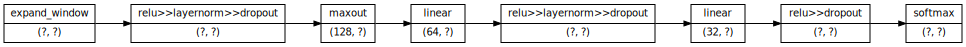
\includegraphics{05_VisualizingThincModels_files/05_VisualizingThincModels_8_0.svg}
\caption{svg}
\end{figure}

Call \mintinline[]{python}{model.initialize} to infer the missing shapes
(using examples of expected input \(X\) and expected output \(Y\)).

\begin{minted}[]{python}
import numpy

X = numpy.zeros(shape=(5, 784), dtype="f")
Y = numpy.zeros(shape=(54000, 10), dtype="f")

model.initialize(X = X, Y = Y)
\end{minted}

\begin{minted}[]{python}
<thinc.model.Model at 0x7f978417da60>
\end{minted}

\begin{minted}[]{python}
visualizeModel(model = model)
\end{minted}

\begin{figure}
\centering
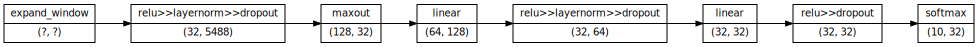
\includegraphics{05_VisualizingThincModels_files/05_VisualizingThincModels_11_0.svg}
\caption{svg}
\end{figure}

\end{document}
